\documentclass{article}
\usepackage{multicol}
\usepackage{lipsum}
\usepackage{lineno}
\usepackage{parskip}

\title{%
Chop Chop \\
  \large Group Report}
\author{
  Connor, Wood\\
  \texttt{cw668}
  \and
  Will, Haysom\\
  \texttt{wah20}
  \and
  Dean, Gooding\\
  \texttt{Dmag2}
  \and
  Beth, Hill\\
  \texttt{Berh2}
  \and
  Jack, Fermer\\
  \texttt{Jdf50}
}

\begin{document}

\maketitle

\pagebreak

\pagenumbering{roman}
\linenumbers

\begin{abstract}
  \addcontentsline{toc}{section}{Abstract}
      This report surrounds our group software development project, a smart cooking assistant called \emph{Chop Chop}. 
    
      In this report we will showcase our group project. We will be evaluating not only the software we made but also how we made it, looking into our design, development, and ways of working. In addition to this, we will 
  \end{abstract}

  \pagebreak

  \tableofcontents

  \pagebreak

  \pagenumbering{arabic}

  %\begin{multicols}{2}

    \section{Introduction}
Chop Chop makes cooking more accessible by offering hands-free, smart recipes. Our smart recipes allow users to get on with cooking without having to worry about looking through the steps of a recipe, scrolling a screen with messy hands, or starting timers. It achieves this by using artificial intelligence, computer vision, and a full-stack application.

    \section{Research}
    \subsection{Object detection}
    Our project's flagship feature was our custom real-time object detection system. This would be used to detect culinary objects such as food and utensils which would dictate when a recipe step had been completed.
    
None of us on the project had experience creating an object detection system. So, we began by doing some research. 

With the huge demand for real-time object detection in the modern age many different algorithms have emerged.

Faster R-CNN offers a real-time object detection algorithm version of R-CNN. “One of the most accurate object detection algorithms” \cite{FasterRCNN} with the drawback of “requires a lot of power at inference time” IE when running in real-time. So, detecting small food objects in a kitchen would be perfect. However, we hoped to run on a Raspberry Pi (a hub in the kitchen area), and we fear the Raspberry Pi will not have the computational power required \cite{Fast-CNN-Rasberry-Pi} at inference time.

Detectron2- Created by Facebook AI research it claims to “provides state-of-the-art detection and segmentation algorithms” \cite{wu2019detectron2} and has been used in many Facebook products such as “Smart Camera for new Portal video-calling devices” \cite{metasmartcameras}. It’s built using the COCO, LVIS, CityScape, and VOC20 datasets, this creates an accurate dataset with an MNAP. However, in many cases “YOLOv8 models outperformed the detectron2 mode” \cite{ai5010005}.

YOLO – You Only Look Once, “It is a state-of-the-art, real-time object detection system which offers extreme levels of speed and accuracy.” \cite{rajeshwari2019object}, that is around “1000x faster than RCNN and 100x faster than the Fast R-CNN model” \cite{rajeshwari2019object}.  It's also shown to have a much higher mAP50-95 "96.7\%" compared to detectron2 (Faster RCNN-101) at "83.554\%"  "YOLO proves to be a cleaner and more efficient" \cite{joiya2022object}, which gave us more confidence if we do eventually choose to run it on slower hardware such as a Raspberry Pi.

Dean reached out to an ex-colleague who had experience in this area. They suggested using YOLOv8 \cite{Jocher_Ultralytics_YOLO_2023} as a base for real-time object detection and suggested using Roboflow \cite{RoboFlow-Software} for dataset management. 

RoboFlow \cite{RoboFlow-Software} is a site where you can easily collaboratively create image datasets. It allows you to upload images you have taken for training, delegate annotation jobs out to different members of the team, and then create a dataset which can be downloaded and trained locally. It was one of the few sites that offered an immense data set (max 10,000 images) with an easy-to-use interface, all for free.

During our research process, we tried out Roboflow and used a trial of their training cloud computers. With only 100 images we were able to confidently detect a Rubik's cube, being held, rotated in the hand, and placed under different backgrounds. Given the lack of experience we had, the relatively small number of images, and the very accurate results we achieved. We were confident that scaling up to whole recipes should on paper be very possible.

    \section{Aims}

    \section{Ways of Working}
    \subsection{Source Control}
    One of the key components to Chop-Chops’ success was our well-set-up and organised GitLab repository. 

    Initially, we decided to create a Gantt chart to record the project timeline and delegate deliverables, which was broken down into two-week sprints. Once all members approved this, it was sent to our supervisor who provided insight into improvements to ensure the project worked effectively. An example of this would be adding our module assessments to the chart to accurately manage and consider our university commitments and workload. 

    A scrum-style agile approach was adopted to our project management strategy. We broke down our Gantt charts’ deliverables into “Issues” on Gitlab. Issues were put on our virtual board, which had four categories, Open, In Development, Review/ Testing, and Closed. These issues were assigned and then moved across given their completion state. 

    From our team’s year-in-industry experience, we adopted a review before merging convention. This rule ensures that tasks were overlooked by other members before being added to the main branch from their working one. This had two main advantages. One was a hugely reduced chance of buggy code getting into the main branch. Two: you gained knowledge of how the rest of the project worked outside of your assigned issues. To enforce this, we locked the main branch from being merged and required at least one approval before the merge.

    We aimed to ensure the main branch was kept as clean as possible; we were mindful of what should and should not be on the repo. This included adding rules to the git ignore file when needed, pruning unnecessary files, and ensuring consistency in naming conventions for files and folders.

    \subsection{Meetings}


    \section{Design}
    \subsection{Frontend}
    Figma was the main tool which we used to craft the frontend design of our web application. We were able to create and pull ideas from each other and prototype how we wanted the design of the application to look by using its collaborative interface. Within this section, we outline our process of exploring and integrating various ideas into our designs, as well as how we utilised Figma to translate these designs into functional code.

    \subsubsection{Research}
    
    Our design process began by investigating and researching what other recipe applications offered in terms of layout, features, and user experience. The three main recipe applications which we focused our research on was BBC Good Foods, AllRecipes and Yummly. 
    
    \paragraph{Recipe Overview}
    Our findings found that the majority of the sites that we looked at showed a featured article or recipe which was the the forefront of the homepage. This component would usually include a background image, title, description, and a button directing users to the featured collection. We quite liked this idea, as it was visually appealing, and an effective way to draw users attention to a focal point on the homepage. We also liked how it could streamline user navigation, and that we could implement our own functionality to make the component work well with our application.
    
    \begin{figure}
      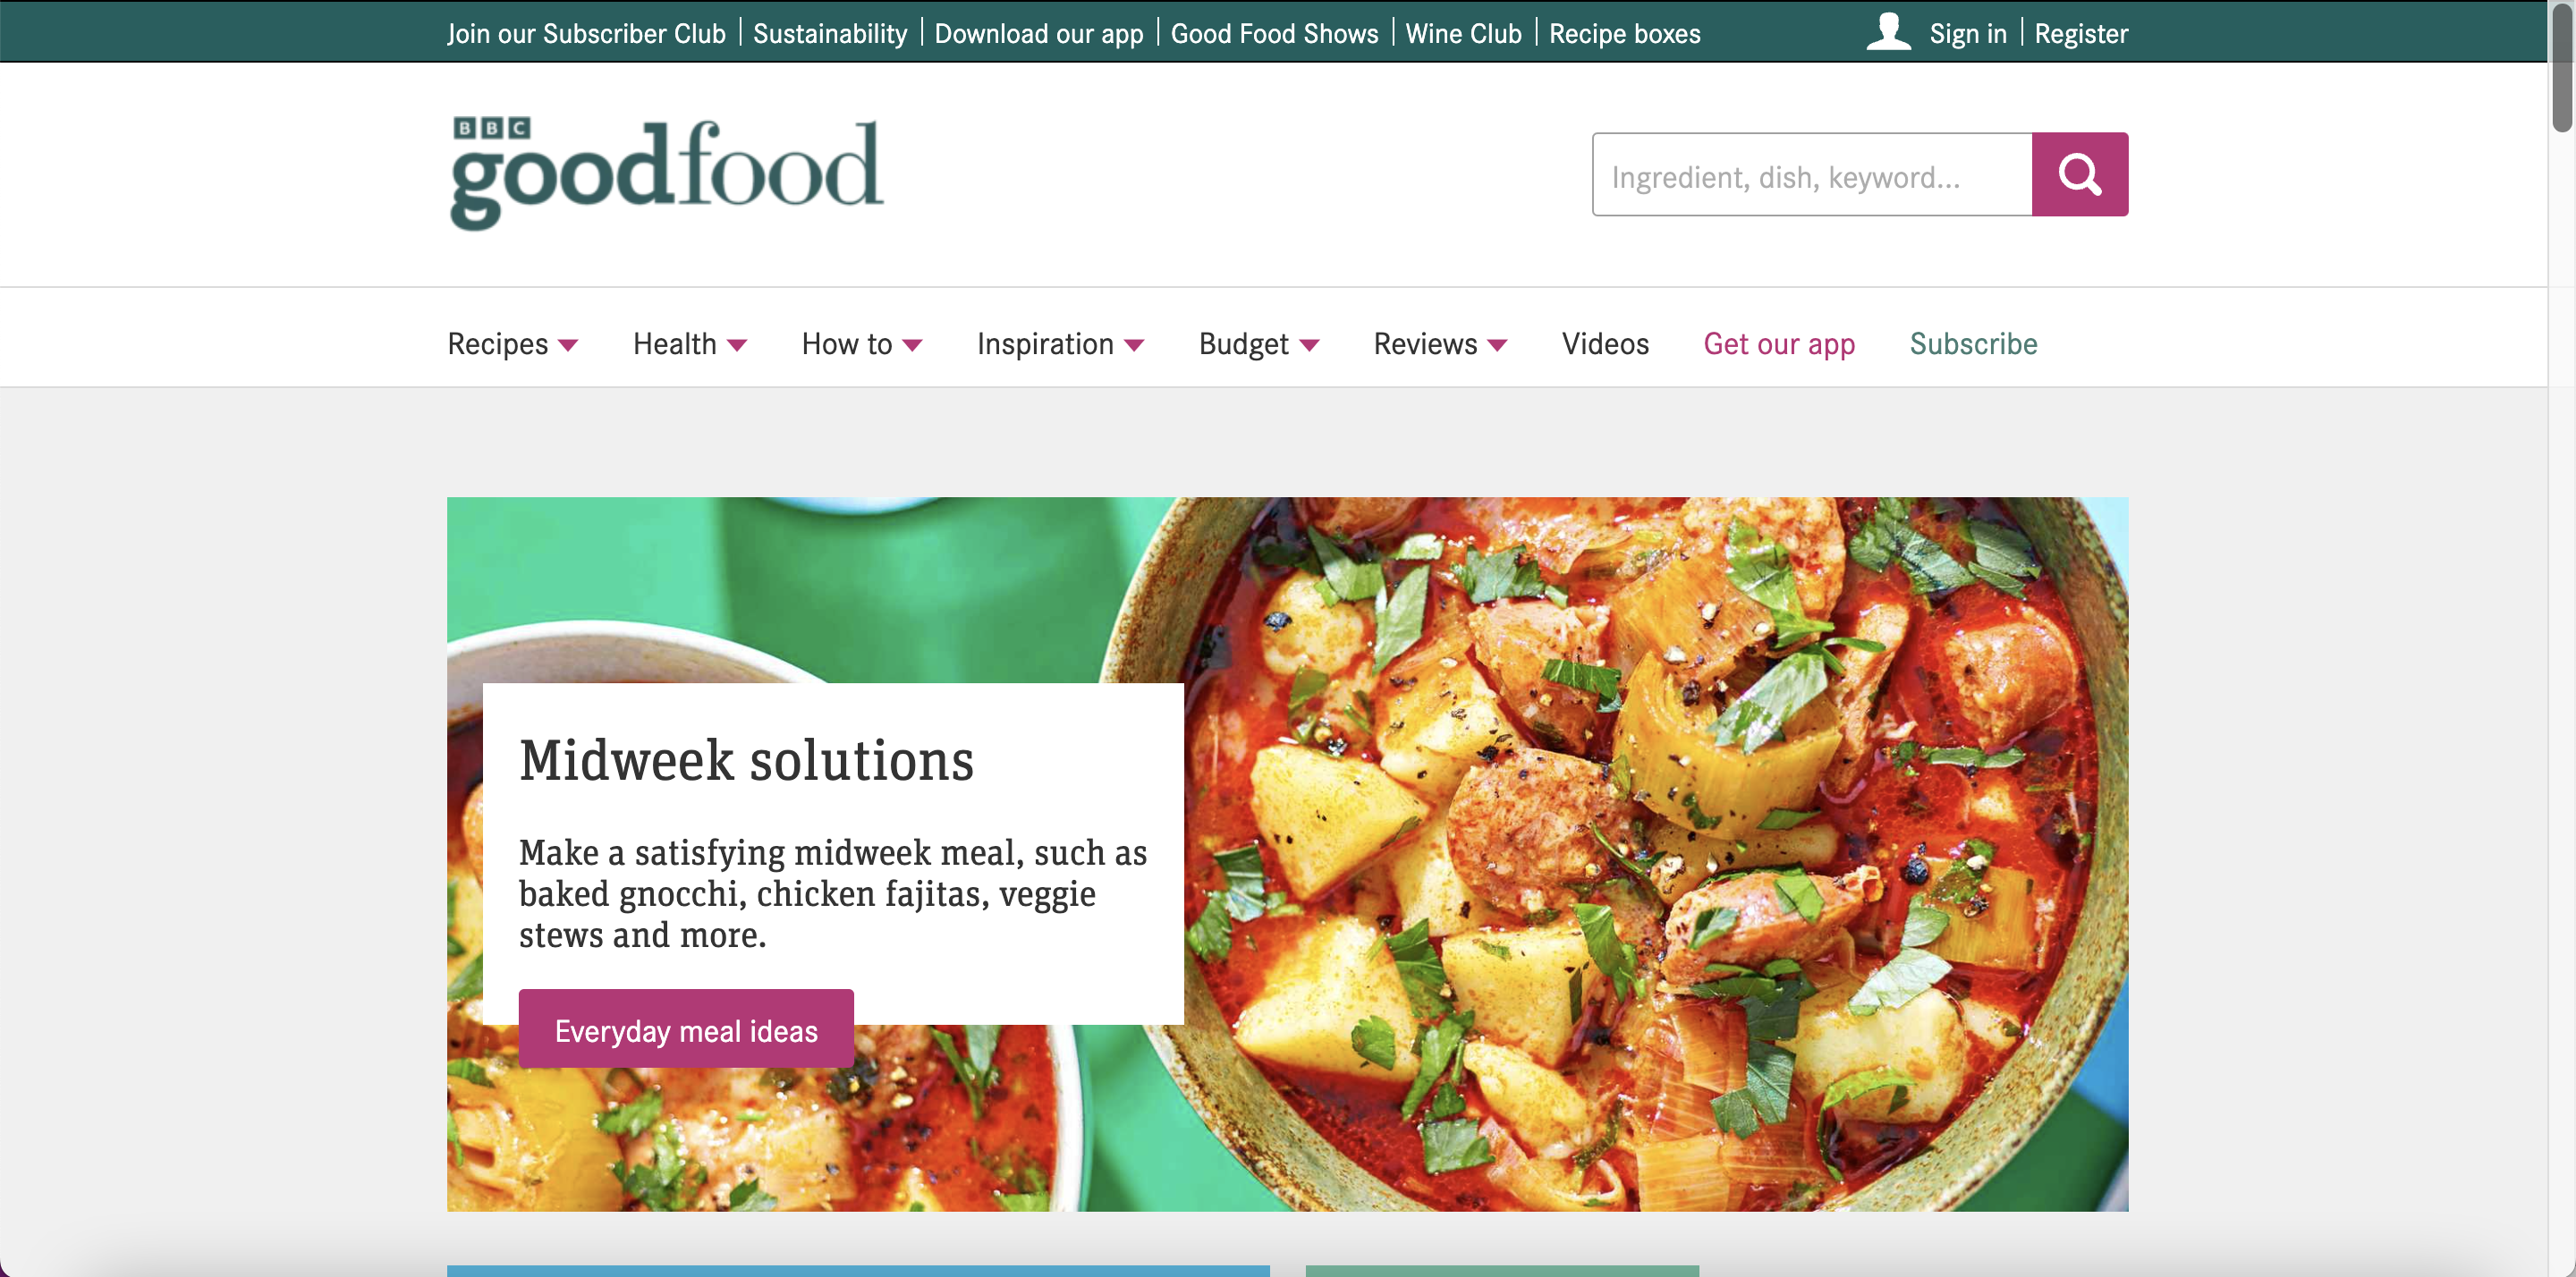
\includegraphics[width=1.0\textwidth]{BBCGF featured-image.png}
      \centering
      \caption{insert caption here}
    \end{figure}

    \paragraph{Recipe cards}
    Each site also used cards as a way to display each recipe. We found that this was an effective way to display each of the recipes, while only showing the necessary information needed for the user.
    
    On Yummly, a variation of their recipe cards caught our attention with an interactive hover feature. Initially displaying just the recipe title, hovering over the card revealed more details about the recipe. We aimed to incorporate a similar functionality into our own cards.
    
    \begin{figure}
      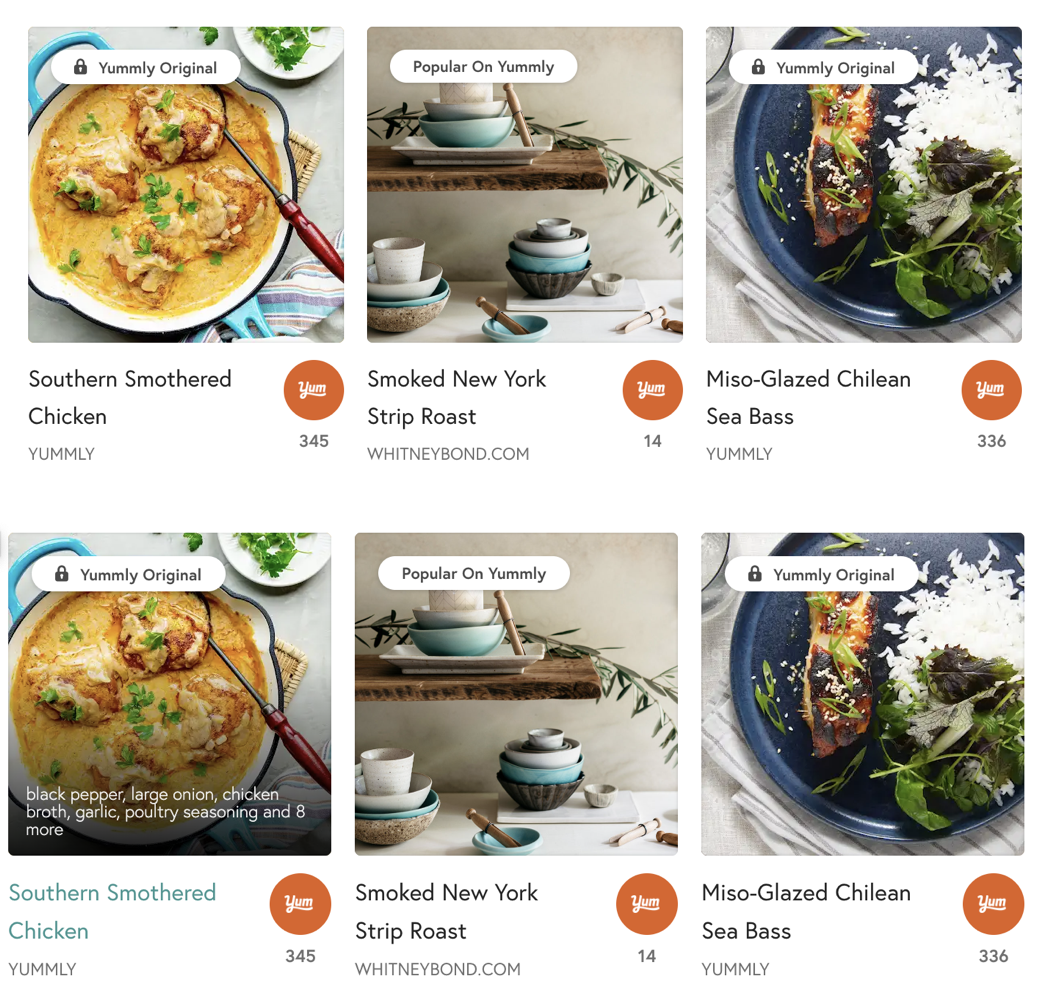
\includegraphics[width=1.0\textwidth]{Yummly recipe cards.png}
      \centering
      \caption{insert caption here}
    \end{figure}

    \paragraph{Recipe Overview}
    For the Recipe Overview page, we wanted the user to be able to see a summary of the recipe and navigate between seeing the recipe steps and the ingredients in a seamless way.
    
    To keep the design of the page simple and clean, we split the page into two sections: the header and the information. The header of the page would show off important information about the recipe, such as the name, a description and a summary of how long the recipe will take to prepare. This section would also feature a start recipe button to take the user to the recipe carousel page.
    
    The information section of the page would showcase both the ingredients and recipe portions of the overview.
    
    After looking at the 3 initial sites, we discovered that the layout was overly cluttered, and the transition between viewing the recipe and its ingredients was not seamless. Instead, most sites placed the ingredients and recipe either side by side or one after the other, which disrupted the flow of navigation.
    
    Instead, we opted for a switcher component that enables users to toggle between viewing the recipe and the ingredients. We believed that this approach would reduce clutter on the page and separate information in a more organised manner. We found inspiration for this functionality on W3Schools.
    
    \begin{figure}
      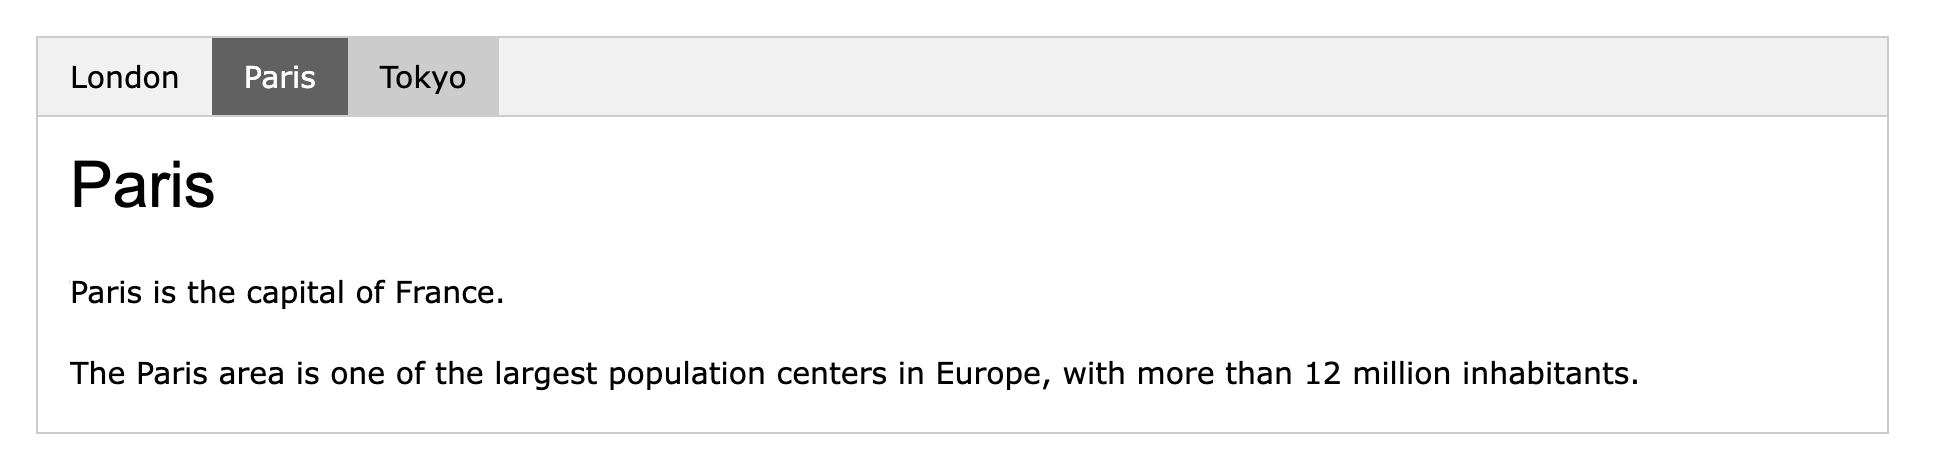
\includegraphics[width=1.0\textwidth]{W3Schools tabbed component.png}
      \centering
      \caption{insert caption here}
    \end{figure}

    We liked the simplicity of this design and the effective functionality to show off information without cluttering the page. 

    \paragraph{Colour Palette}
    To begin our investigation into which colour palette should be used for the frontend, we decided to investigate any accessibility issues which we will have to take in to consideration to ensure that our design enhanced readability and usability for all users. 

    During this investigation, we found that the use of bright colours may cause pain for those who suffer with low vision or dyslexia, and may also prevent them from being able to read information from the page. This means that websites need to have a low brightness background to accommodate for this disability.
    
    Users also need a high contrast between the text and the background on a page. According to the W3C accessibility standards, people will be able to read information better on a page which incorporates dark text on a light background. We wanted to select colours for our frontend which would meet both of these accessibility criteria and found that a neutral tone for our main colour scheme would effectively meet these standards.
    
    For the background of the the web application, we opted to use a pale peach colour. We selected this colour as it would provide a warmth to the page while also ensuring that users who struggle with bright backgrounds are not overwhelmed when reading information. Furthermore, the selection of this colour made it easier to find secondary colours for text and highlights that would provide a bold contrast.

    \subsubsection{Figma vs Zeplin}
    Before we began to design the prototype of the frontend, we had to decide which software application we should use. From prior experience during our placement year, we initially chose to use either Figma or Zeplin.

    Within our research, we found that Zeplin is primarily a collaboration and handoff tool whereas Figma is a comprehensive design tool that enables collaborative design, prototyping, and sharing within a single platform. This means that you could create designs directly using Figma, while on Zeplin, designs must be created using a dedicated design tool such as Sketch or Adobe XD, and then imported. 
    
    Figma also features a Dev Mode interface that allows for developers to translate created designs into code more efficiently. As a team, we liked the use of this feature since we would be able to streamline the design-to-development workflow and reduce the use of repetitive, manual coding.
    
    While Zeplin does also feature some developer tools, Figma is exclusively tailored for the design process. This means that Figma can provide a better experience while designing prototypes as it doe not have the additional complexity of features which are shown within Zeplin. 

    After considering the pros and cons of both applications, combined with the research which we conducted, we decided that Figma would be the best solution for us.
    

    \subsection{Architecture}
  

    \section{Development}
    \subsection{Backend}

    \subsection{Frontend}
 
    \subsection{Database}

    \subsection{Data Collection \& Training}
    \subsubsection{RoboFlow}
    For developing our object detection system, we needed a trained model. From our research, we decided to use Roboflow for data collection and management and trained with YOLOv8.
    
To train, we first needed to collect many images of the object we wanted to detect. We found during development that it is best to start with lots of good-quality images of the object; They should be in good lighting and well-framed. Then many different positions of objects in the frame. Finally, gathering some more obscure images. These can be in different lighting conditions, from far away, and with multiple other objects in the frame as well. These all create a diverse data set, which increases the chance of detection.

Once a significant number of images had been gathered (around 100) they were uploaded to Roboflow for annotating. Annotation jobs can be generated and sent to each person on the project. We decided to use box annotation, as it was significantly quicker to annotate and in our preliminary tests offered the same level of object detection that poly-selection did.

Each annotation was then reviewed by someone else before being added to the dataset. This ensured that the dataset was accurate in its annotations as small mistakes could teach the AI the wrong classification.

When all images are annotated a new YOLOv8 dataset can be generated. Before this Roboflow will split up your images into training, testing, and validation. Training will teach AI, validation are used to as it trains test how good the AI is getting. Testing “a test data set is a separate sample, an unseen data set, to provide an unbiased final evaluation of a model fit.” \cite{trainvalidtest} It will resize the image to 640x640 which greatly reduces training time, and smaller images reduce computational cost. 

Finally, it generates extra images through augmentation. We chose Shear ±15° and Brightness ±25\%. Shear would simulate different camera angles, which would provide greater angle coverage. Brightness would widen the number of handled lighting conditions, as different kitchens could have very varied levels of brightness.

    \subsubsection{Training with CUDA}
    

    


    \section{Testing}

    \section{Results}

    \section{Future Work}

    \section{Conclusion}

    \pagebreak

    
  %\end{multicols}
  
  \addcontentsline{toc}{section}{References}

  \bibliographystyle{ieeetr}
  
  \bibliography{group-doc}

\end{document}